Físicamente, el proceso de siembra de una semilla dada puede llevarse a cabo cualquier día del año, especialmente cuando se tienen las condiciones climáticas adecuadas \cite{Qiao_2023}. De igual manera, la fecha de siembra constituye una práctica de manejo agrícola fundamental, ya que determina las condiciones ambientales que experimentará el cultivo a lo largo de su desarrollo \cite{Sadeh_2024}.\\

Históricamente, muchas de las prácticas agrícolas se consolidaron mediante procesos empíricos de observación y ajuste progresivo en los cuales, a través de ensayo y error, se identificaban los periodos más favorables; por ejemplo, para la siembra \cite{NRC_1996}. En el contexto actual, este tipo de decisiones debe replantearse dado que las condiciones en las que fueron tomadas se han alterado por la incertidumbre y la variabilidad asociadas al cambio climático.\\

En este sentido, se propone una metodología probabilística que formaliza este proceso empírico de exploración del calendario agrícola, permitiendo estudiar analíticamente la variabilidad temporal de las fechas de siembra y estimar periodos potencialmente favorables para el establecimiento del cultivo bajo condiciones climáticas variables.\\


Más aún, se estructura la progresión del tiempo como un proceso cíclico, emulando  la periodicidad inherente a la naturaleza \cite{Chuine_2017,Gatto_2015,Gurney_1992,Mardia1999,Powell_2005,Regniere_2013}, ver Fig. \ref{Transicion}. De esta manera, supongamos que una semilla de maíz será sembrada en campo abierto si tal semilla no es viable entonces se concluye el proceso de siembra como fallido. En otro caso, si dicha semilla es viable y se siembra el día $D_i$, para alguna $i\in\{1,2,3,\ldots, 365\}$ el proceso puede concluir con la emergencia o con el fracaso al día $D_j$, para alguna $j\geq i$, $j\mod{365} \in \{1,2,3,\ldots, 365\}$.\\

Por convención, definamos 
	\begin{align}
		D_{366}\coloneqq& D_{1},\\
		D_{367}\coloneqq& D_{2},\\
		\nonumber\vdots& \\
		D_{j}\coloneqq& D_{j\mod{365}}.
	\end{align}
Con lo anterior, es posible dotar de una estructura cíclica a la progresión del año dado que al finalizar un año inmediatamente comienza el siguiente de manera que la observación del proceso de siembra puede observarse de manera continua en todo punto del año.\\

Sea $n^*\in \N$ el número de días necesarios para que una semilla viable de maíz logre la emergencia desde su siembra. Como se busca determinar los periodos en donde las condiciones agroambientales favorezcan un sano desarrollo de la semilla, reduciendo la exposición al estrés del entorno entonces se desea hallar al conjunto de días $D_i$ tales que una semilla sembrada en dicha fecha emerja al día $D_{i+n^*}$ con una probabilidad \textit{suficientemente grande}.\\

Sea $X=\{X_t\}_{t\in \N}$ un proceso estocástico a tiempo discreto y con espacio de estados $S=\{D_1, D_2,\ldots, D_{365}, F\}$ tal que la variable aleatoria $X_t$ modela el desarrollo de la semilla al $t$-ésimo día de ser sembrada. Asimismo, el estado $F$ indica el fracaso mientras que los estados $D_i$ indican un correcto crecimiento al $i$-ésimo día del año.\\

De esta manera, dado dos estados $i,j\in S$, $i\neq j$ si $P_{i,j}$ denota la probabilidad de partir del estado $i$ para transicionar al estado $j$, en un paso, entonces \begin{equation}
	P_{i, j} \coloneqq P(X_{t+1}= j\mid X_{t}= i ) = 
	\begin{cases}
		\lambda_k, \text{ si } i=D_k \text{ y } j= D_{k+1}, k\in \{1,2,\ldots,365\}.\\
		1-\lambda_k, \text{ si } i=D_k, k\in \{1,2,\ldots,365\}, \text{ y } j= F.\\
		1, \text{ si } i=F \text{ y } j= F.\\
		0, \text{ en otro caso.}
	\end{cases}
	\label{TransitionProbs}
\end{equation}
Donde, para cada $k\in \{1,2,\ldots, 365\}$, \begin{equation}
	\lambda_k= 1- \frac{d(C_{H,k} \,\mathbf{,}\, C^*)}{\displaystyle \max_{l\in \{1,\ldots, 365\}} \{d(C_{H,l}\, \mathbf{,} \,C^*)\}}.
\end{equation}Además, $C_{H,k}$ denota el centroide de las condiciones agroambientales históricas registradas el $k$-ésimo día del año mientras que $C^*$ denota el centroide de la región de condiciones agroambientales óptimas para el desarrollo del maíz, ver Fig. \ref{Distance}.\\

\tikzset{every picture/.style={line width=0.75pt}} %set default line width to 0.75pt        
\begin{figure}[ht]
	\centering
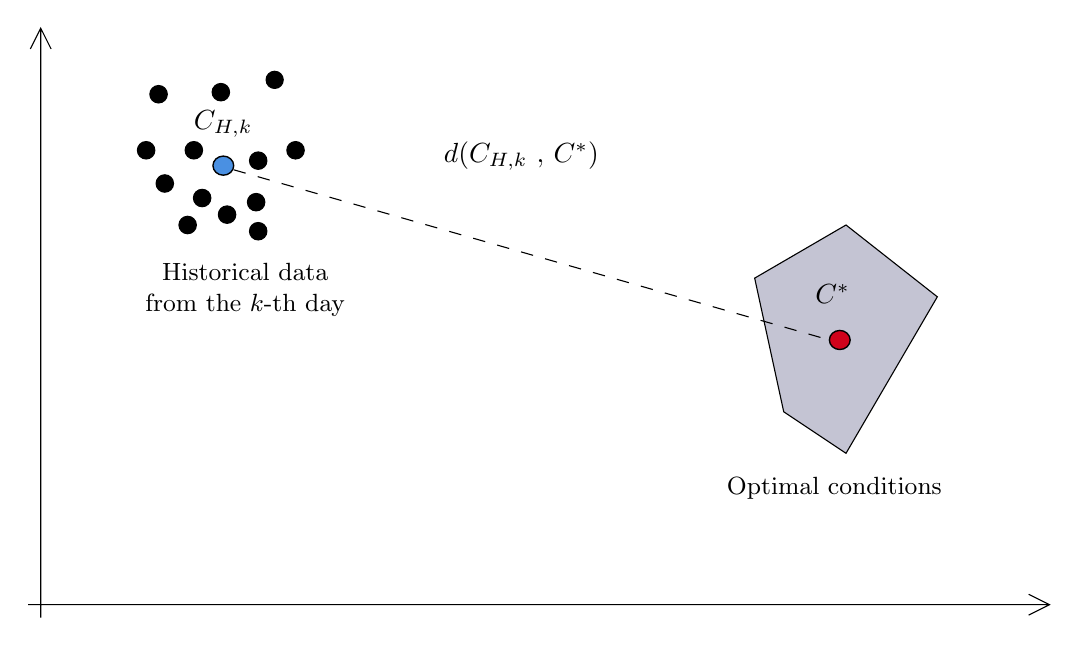
\begin{tikzpicture}[x=0.75pt,y=0.75pt,yscale=-1,xscale=1]
	%uncomment if require: \path (0,717); %set diagram left start at 0, and has height of 717
	
	%Shape: Axis 2D [id:dp4496072713140289] 
	\draw  (58,700.13) -- (550,700.13)(64.03,422.4) -- (64.03,706.4) (540,695.13) -- (550,700.13) -- (540,705.13) (59.03,432.4) -- (64.03,422.4) -- (69.03,432.4)  ;
	%Shape: Circle [id:dp06215554504361531] 
	\draw  [fill={rgb, 255:red, 0; green, 0; blue, 0 }  ,fill opacity=1 ] (133.6,481.2) .. controls (133.6,478.88) and (135.48,477) .. (137.8,477) .. controls (140.12,477) and (142,478.88) .. (142,481.2) .. controls (142,483.52) and (140.12,485.4) .. (137.8,485.4) .. controls (135.48,485.4) and (133.6,483.52) .. (133.6,481.2) -- cycle ;
	%Shape: Circle [id:dp22652234947291816] 
	\draw  [fill={rgb, 255:red, 0; green, 0; blue, 0 }  ,fill opacity=1 ] (182.6,481.2) .. controls (182.6,478.88) and (184.48,477) .. (186.8,477) .. controls (189.12,477) and (191,478.88) .. (191,481.2) .. controls (191,483.52) and (189.12,485.4) .. (186.8,485.4) .. controls (184.48,485.4) and (182.6,483.52) .. (182.6,481.2) -- cycle ;
	%Shape: Circle [id:dp7411954551562622] 
	\draw  [fill={rgb, 255:red, 0; green, 0; blue, 0 }  ,fill opacity=1 ] (172.6,447.26) .. controls (172.6,444.98) and (174.45,443.13) .. (176.74,443.13) .. controls (179.02,443.13) and (180.87,444.98) .. (180.87,447.26) .. controls (180.87,449.55) and (179.02,451.4) .. (176.74,451.4) .. controls (174.45,451.4) and (172.6,449.55) .. (172.6,447.26) -- cycle ;
	%Shape: Circle [id:dp9342194323542646] 
	\draw  [fill={rgb, 255:red, 0; green, 0; blue, 0 }  ,fill opacity=1 ] (110.6,481.2) .. controls (110.6,478.88) and (112.48,477) .. (114.8,477) .. controls (117.12,477) and (119,478.88) .. (119,481.2) .. controls (119,483.52) and (117.12,485.4) .. (114.8,485.4) .. controls (112.48,485.4) and (110.6,483.52) .. (110.6,481.2) -- cycle ;
	%Shape: Circle [id:dp7509634202671536] 
	\draw  [fill={rgb, 255:red, 0; green, 0; blue, 0 }  ,fill opacity=1 ] (130.6,517.2) .. controls (130.6,514.88) and (132.48,513) .. (134.8,513) .. controls (137.12,513) and (139,514.88) .. (139,517.2) .. controls (139,519.52) and (137.12,521.4) .. (134.8,521.4) .. controls (132.48,521.4) and (130.6,519.52) .. (130.6,517.2) -- cycle ;
	%Shape: Circle [id:dp3389656361514962] 
	\draw  [fill={rgb, 255:red, 0; green, 0; blue, 0 }  ,fill opacity=1 ] (119.6,497.2) .. controls (119.6,494.88) and (121.48,493) .. (123.8,493) .. controls (126.12,493) and (128,494.88) .. (128,497.2) .. controls (128,499.52) and (126.12,501.4) .. (123.8,501.4) .. controls (121.48,501.4) and (119.6,499.52) .. (119.6,497.2) -- cycle ;
	%Shape: Circle [id:dp7223141295117336] 
	\draw  [fill={rgb, 255:red, 0; green, 0; blue, 0 }  ,fill opacity=1 ] (149.6,512.2) .. controls (149.6,509.88) and (151.48,508) .. (153.8,508) .. controls (156.12,508) and (158,509.88) .. (158,512.2) .. controls (158,514.52) and (156.12,516.4) .. (153.8,516.4) .. controls (151.48,516.4) and (149.6,514.52) .. (149.6,512.2) -- cycle ;
	%Shape: Circle [id:dp7582728872550809] 
	\draw  [fill={rgb, 255:red, 0; green, 0; blue, 0 }  ,fill opacity=1 ] (116.6,454.2) .. controls (116.6,451.88) and (118.48,450) .. (120.8,450) .. controls (123.12,450) and (125,451.88) .. (125,454.2) .. controls (125,456.52) and (123.12,458.4) .. (120.8,458.4) .. controls (118.48,458.4) and (116.6,456.52) .. (116.6,454.2) -- cycle ;
	%Shape: Circle [id:dp49904732080555536] 
	\draw  [fill={rgb, 255:red, 0; green, 0; blue, 0 }  ,fill opacity=1 ] (163.6,506.2) .. controls (163.6,503.88) and (165.48,502) .. (167.8,502) .. controls (170.12,502) and (172,503.88) .. (172,506.2) .. controls (172,508.52) and (170.12,510.4) .. (167.8,510.4) .. controls (165.48,510.4) and (163.6,508.52) .. (163.6,506.2) -- cycle ;
	%Shape: Circle [id:dp9713308312029804] 
	\draw  [fill={rgb, 255:red, 0; green, 0; blue, 0 }  ,fill opacity=1 ] (164.6,486.2) .. controls (164.6,483.88) and (166.48,482) .. (168.8,482) .. controls (171.12,482) and (173,483.88) .. (173,486.2) .. controls (173,488.52) and (171.12,490.4) .. (168.8,490.4) .. controls (166.48,490.4) and (164.6,488.52) .. (164.6,486.2) -- cycle ;
	%Shape: Circle [id:dp6213316985023771] 
	\draw  [fill={rgb, 255:red, 0; green, 0; blue, 0 }  ,fill opacity=1 ] (164.6,520.2) .. controls (164.6,517.88) and (166.48,516) .. (168.8,516) .. controls (171.12,516) and (173,517.88) .. (173,520.2) .. controls (173,522.52) and (171.12,524.4) .. (168.8,524.4) .. controls (166.48,524.4) and (164.6,522.52) .. (164.6,520.2) -- cycle ;
	%Shape: Polygon [id:ds0377823447882647] 
	\draw [fill={rgb, 255:red, 20; green, 20; blue, 80 }  ,fill opacity=0.25 ] (452,517.2) -- (496,551.8) -- (452,627.2) -- (422,607.2) -- (408,542.8) -- cycle ;
	%Flowchart: Summing Junction [id:dp4210872697663528] 
	\draw  [fill={rgb, 255:red, 74; green, 144; blue, 226 }  ,fill opacity=1 ][line width=0.5]  (147,488.6) .. controls (147,486.06) and (149.24,484) .. (152,484) .. controls (154.76,484) and (157,486.06) .. (157,488.6) .. controls (157,491.14) and (154.76,493.2) .. (152,493.2) .. controls (149.24,493.2) and (147,491.14) .. (147,488.6) -- cycle ;% \draw  [line width=1.5]  (148.46,485.35) -- (155.54,491.85) ; \draw  [line width=1.5]  (155.54,485.35) -- (148.46,491.85) ;
	%Shape: Circle [id:dp3856640767966395] 
	\draw  [fill={rgb, 255:red, 0; green, 0; blue, 0 }  ,fill opacity=1 ] (137.6,504.2) .. controls (137.6,501.88) and (139.48,500) .. (141.8,500) .. controls (144.12,500) and (146,501.88) .. (146,504.2) .. controls (146,506.52) and (144.12,508.4) .. (141.8,508.4) .. controls (139.48,508.4) and (137.6,506.52) .. (137.6,504.2) -- cycle ;
	%Flowchart: Summing Junction [id:dp21052777836013448] 
	\draw  [fill={rgb, 255:red, 208; green, 2; blue, 27 }  ,fill opacity=1 ][line width=0.5]  (444,572.6) .. controls (444,570.06) and (446.24,568) .. (449,568) .. controls (451.76,568) and (454,570.06) .. (454,572.6) .. controls (454,575.14) and (451.76,577.2) .. (449,577.2) .. controls (446.24,577.2) and (444,575.14) .. (444,572.6) -- cycle ; %\draw  [line width=1.5]  (445.46,569.35) -- (452.54,575.85) ; \draw  [line width=1.5]  (452.54,569.35) -- (445.46,575.85) ;
	%Straight Lines [id:da05984024528227749] 
	\draw  [dash pattern={on 4.5pt off 4.5pt}]  (157,490.6) -- (444,572.6) ;
	%Shape: Circle [id:dp618933165821857] 
	\draw  [fill={rgb, 255:red, 0; green, 0; blue, 0 }  ,fill opacity=1 ] (146.6,453.2) .. controls (146.6,450.88) and (148.48,449) .. (150.8,449) .. controls (153.12,449) and (155,450.88) .. (155,453.2) .. controls (155,455.52) and (153.12,457.4) .. (150.8,457.4) .. controls (148.48,457.4) and (146.6,455.52) .. (146.6,453.2) -- cycle ;
	
	% Text Node
	\draw (104,534.4) node [anchor=north west][inner sep=0.75pt]  [font=\small] [align=left] {\begin{minipage}[lt]{85.87pt}\setlength\topsep{0pt}
			\begin{center}
				Historical data\\from the $k$-th day
			\end{center}
			
	\end{minipage}};
	% Text Node
	\draw (393,637.4) node [anchor=north west][inner sep=0.75pt]  [font=\small] [align=left] {\begin{minipage}[lt]{78.21pt}\setlength\topsep{0pt}
			\begin{center}
				Optimal conditions
			\end{center}
			
	\end{minipage}};
	% Text Node
	\draw (136.6,460.6) node [anchor=north west][inner sep=0.75pt]    {$C_{H,k}$};
	% Text Node
	\draw (436,544.4) node [anchor=north west][inner sep=0.75pt]    {$C^*$};
	% Text Node
	\draw (257,475.8) node [anchor=north west][inner sep=0.75pt]    {$d( C_{H,k} \ \mathbf{,}\ C^*)$};
	% Text Node
	%\draw (100,362.8) node [anchor=north west][inner sep=0.75pt]    {$P( X_{t+1} =D_{k+1} \mid X_{t} =D_{k}) \coloneq \ 1-\frac{\displaystyle d( C_{H,k} \ ,\ C_{O})}{\displaystyle\max_{l\in \{1,2,\dots, 365\}} \ \{d( C_{H,l} \ ,\ C_{O})\}} \ =\ \lambda _{k}.$};
\end{tikzpicture}
\caption{Distancia entre las condiciones agroclimáticas para el desarrollo óptimo del maíz y las condiciones agroclimáticas históricamente reportadas para el $k$-ésimo día del año. Los círculos en color negro representan los datos agroclimáticos reportados anualmente para el $k$-ésimo día del año mientras que el polígono sombreado en color gris representa la región de parámetros agroclimáticos, ideales para el desarrollo del maíz. Los círculos de color azul y rojo indican los centroides de los datos históricos ($C_{H,k}$) y la región óptima ($C^*$), respectivamente.}
\label{Distance}
\end{figure}

Para ilustrar lo discutido en la Ecuación \eqref{TransitionProbs}, se construyó un diagrama de transición
en donde se muestra tanto la estructura cíclica como proceso estocástico que subyacen en la modelación del problema, ver Fig. \ref{Transicion}.

\begin{figure}[ht]
	\centering
	\resizebox{0.75\textwidth}{!}{
	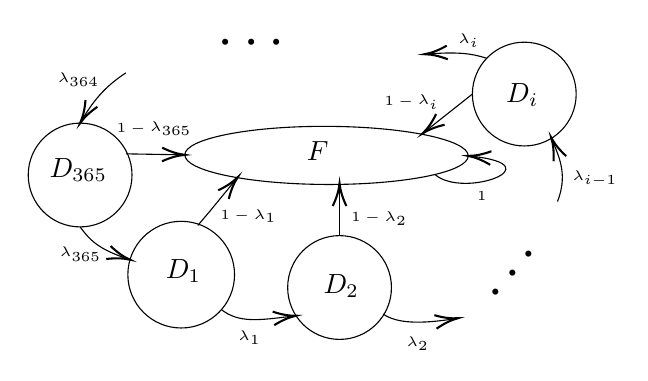
\begin{tikzpicture}[x=0.75pt,y=0.75pt,yscale=-1,xscale=1]
		%uncomment if require: \path (0,300); %set diagram left start at 0, and has height of 300
		
		%Shape: Circle [id:dp8593186993316585] 
		\draw   (84,153.8) .. controls (84,139.99) and (95.19,128.8) .. (109,128.8) .. controls (122.81,128.8) and (134,139.99) .. (134,153.8) .. controls (134,167.61) and (122.81,178.8) .. (109,178.8) .. controls (95.19,178.8) and (84,167.61) .. (84,153.8) -- cycle ;
		%Shape: Circle [id:dp4933341749796484] 
		\draw   (132,201.8) .. controls (132,187.61) and (143.51,176.1) .. (157.7,176.1) .. controls (171.89,176.1) and (183.4,187.61) .. (183.4,201.8) .. controls (183.4,215.99) and (171.89,227.5) .. (157.7,227.5) .. controls (143.51,227.5) and (132,215.99) .. (132,201.8) -- cycle ;
		%Shape: Circle [id:dp8064812302387944] 
		\draw   (209,208) .. controls (209,194.19) and (220.19,183) .. (234,183) .. controls (247.81,183) and (259,194.19) .. (259,208) .. controls (259,221.81) and (247.81,233) .. (234,233) .. controls (220.19,233) and (209,221.81) .. (209,208) -- cycle ;
		%Shape: Circle [id:dp5691763998987368] 
		\draw   (298,114.8) .. controls (298,100.99) and (309.19,89.8) .. (323,89.8) .. controls (336.81,89.8) and (348,100.99) .. (348,114.8) .. controls (348,128.61) and (336.81,139.8) .. (323,139.8) .. controls (309.19,139.8) and (298,128.61) .. (298,114.8) -- cycle ;
		%Curve Lines [id:da4516456787286707] 
		\draw    (109,178.8) .. controls (113.8,185.33) and (117.68,189.28) .. (131.25,194) ;
		\draw [shift={(133,194.6)}, rotate = 198.43] [color={rgb, 255:red, 0; green, 0; blue, 0 }  ][line width=0.75]    (10.93,-3.29) .. controls (6.95,-1.4) and (3.31,-0.3) .. (0,0) .. controls (3.31,0.3) and (6.95,1.4) .. (10.93,3.29)   ;
		%Curve Lines [id:da212037411386651] 
		\draw    (177,218.6) .. controls (185.69,225.35) and (195.3,223.73) .. (211.24,221.81) ;
		\draw [shift={(213,221.6)}, rotate = 173.29] [color={rgb, 255:red, 0; green, 0; blue, 0 }  ][line width=0.75]    (10.93,-3.29) .. controls (6.95,-1.4) and (3.31,-0.3) .. (0,0) .. controls (3.31,0.3) and (6.95,1.4) .. (10.93,3.29)   ;
		%Curve Lines [id:da6785657414733032] 
		\draw    (339,166.6) .. controls (343.7,154.38) and (340.45,146.58) .. (336.72,137.55) ;
		\draw [shift={(336,135.8)}, rotate = 67.8] [color={rgb, 255:red, 0; green, 0; blue, 0 }  ][line width=0.75]    (10.93,-3.29) .. controls (6.95,-1.4) and (3.31,-0.3) .. (0,0) .. controls (3.31,0.3) and (6.95,1.4) .. (10.93,3.29)   ;
		%Curve Lines [id:da24911935793481532] 
		\draw    (131,104.6) .. controls (122.41,110.33) and (116.55,116.06) .. (109.94,127.19) ;
		\draw [shift={(109,128.8)}, rotate = 299.85] [color={rgb, 255:red, 0; green, 0; blue, 0 }  ][line width=0.75]    (10.93,-3.29) .. controls (6.95,-1.4) and (3.31,-0.3) .. (0,0) .. controls (3.31,0.3) and (6.95,1.4) .. (10.93,3.29)   ;
		%Curve Lines [id:da18281523000825994] 
		\draw    (255,220.8) .. controls (261.76,225.43) and (273.17,225.59) .. (289.23,223.08) ;
		\draw [shift={(291,222.8)}, rotate = 170.65] [color={rgb, 255:red, 0; green, 0; blue, 0 }  ][line width=0.75]    (10.93,-3.29) .. controls (6.95,-1.4) and (3.31,-0.3) .. (0,0) .. controls (3.31,0.3) and (6.95,1.4) .. (10.93,3.29)   ;
		%Shape: Ellipse [id:dp9200963781142645] 
		\draw   (159.44,144.1) .. controls (159.47,136.37) and (190.06,130.21) .. (227.77,130.35) .. controls (265.48,130.49) and (296.03,136.87) .. (296,144.6) .. controls (295.97,152.33) and (265.38,158.49) .. (227.67,158.35) .. controls (189.96,158.21) and (159.41,151.83) .. (159.44,144.1) -- cycle ;
		%Straight Lines [id:da4255411591292486] 
		\draw    (131,143.6) -- (157.44,144.06) ;
		\draw [shift={(159.44,144.1)}, rotate = 181.01] [color={rgb, 255:red, 0; green, 0; blue, 0 }  ][line width=0.75]    (10.93,-3.29) .. controls (6.95,-1.4) and (3.31,-0.3) .. (0,0) .. controls (3.31,0.3) and (6.95,1.4) .. (10.93,3.29)   ;
		%Straight Lines [id:da3690504090862228] 
		\draw    (234,183) -- (234,159.8) ;
		\draw [shift={(234,157.8)}, rotate = 90] [color={rgb, 255:red, 0; green, 0; blue, 0 }  ][line width=0.75]    (10.93,-3.29) .. controls (6.95,-1.4) and (3.31,-0.3) .. (0,0) .. controls (3.31,0.3) and (6.95,1.4) .. (10.93,3.29)   ;
		%Straight Lines [id:da2286251332217033] 
		\draw    (165.7,178.1) -- (171.44,171.33) -- (183.73,156.35) ;
		\draw [shift={(185,154.8)}, rotate = 129.36] [color={rgb, 255:red, 0; green, 0; blue, 0 }  ][line width=0.75]    (10.93,-3.29) .. controls (6.95,-1.4) and (3.31,-0.3) .. (0,0) .. controls (3.31,0.3) and (6.95,1.4) .. (10.93,3.29)   ;
		%Curve Lines [id:da9498383507436814] 
		\draw    (305,97.6) .. controls (296.45,94.75) and (288.8,94.61) .. (276.91,95.46) ;
		\draw [shift={(275,95.6)}, rotate = 355.6] [color={rgb, 255:red, 0; green, 0; blue, 0 }  ][line width=0.75]    (10.93,-3.29) .. controls (6.95,-1.4) and (3.31,-0.3) .. (0,0) .. controls (3.31,0.3) and (6.95,1.4) .. (10.93,3.29)   ;
		%Straight Lines [id:da19016244462240628] 
		\draw    (298,114.8) -- (275.57,132.56) ;
		\draw [shift={(274,133.8)}, rotate = 321.63] [color={rgb, 255:red, 0; green, 0; blue, 0 }  ][line width=0.75]    (10.93,-3.29) .. controls (6.95,-1.4) and (3.31,-0.3) .. (0,0) .. controls (3.31,0.3) and (6.95,1.4) .. (10.93,3.29)   ;
		%Curve Lines [id:da5763736584575927] 
		\draw    (280,153.6) .. controls (293.79,165.42) and (337.66,149.1) .. (297.88,144.79) ;
		\draw [shift={(296,144.6)}, rotate = 5.31] [color={rgb, 255:red, 0; green, 0; blue, 0 }  ][line width=0.75]    (10.93,-3.29) .. controls (6.95,-1.4) and (3.31,-0.3) .. (0,0) .. controls (3.31,0.3) and (6.95,1.4) .. (10.93,3.29)  ;
		% Text Node INFERIOR
		\draw (300.98,209.85) node [anchor=north west][inner sep=0.75pt]  [font=\huge,rotate=-310.72]  {$\cdots $};
		% Text Node
		\draw (149,193.4) node [anchor=north west][inner sep=0.75pt]    {$D_{1}$};
		% Text Node
		\draw (225,200.4) node [anchor=north west][inner sep=0.75pt]    {$D_{2}$};
		% Text Node
		\draw (313,108.4) node [anchor=north west][inner sep=0.75pt]    {$D_{i}$};
		% Text Node
		\draw (93,144.4) node [anchor=north west][inner sep=0.75pt]    {$D_{365}$};
		% Text Node sUPERIOR
		\draw (174.21,83.08) node [anchor=north west][inner sep=0.75pt]  [font=\huge,rotate=-0.63]  {$\cdots $};
		% Text Node
		\draw (184,227.4) node [anchor=north west][inner sep=0.75pt]  [font=\tiny]  {$\lambda _{1}$};
		% Text Node
		\draw (175.28,169.43) node [anchor=north west][inner sep=0.75pt]  [font=\tiny,rotate=-358.96]  {$1-\lambda _{1}$};
		% Text Node
		\draw (265,230.4) node [anchor=north west][inner sep=0.75pt]  [font=\tiny]  {$\lambda _{2}$};
		% Text Node
		\draw (345,150.4) node [anchor=north west][inner sep=0.75pt]  [font=\tiny]  {$\lambda _{i-1}$};
		% Text Node
		\draw (98,187.4) node [anchor=north west][inner sep=0.75pt]  [font=\tiny]  {$\lambda _{365}$};
		% Text Node
		\draw (97,103.4) node [anchor=north west][inner sep=0.75pt]  [font=\tiny]  {$\lambda _{364}$};
		% Text Node
		\draw (290,84.4) node [anchor=north west][inner sep=0.75pt]  [font=\tiny]  {$\lambda _{i}$};
		% Text Node
		\draw (238.28,170.43) node [anchor=north west][inner sep=0.75pt]  [font=\tiny,rotate=-358.96]  {$1-\lambda _{2}$};
		% Text Node
		\draw (254.28,114.43) node [anchor=north west][inner sep=0.75pt]  [font=\tiny,rotate=-358.96]  {$1-\lambda _{i}$};
		% Text Node
		\draw (125.28,127.43) node [anchor=north west][inner sep=0.75pt]  [font=\tiny,rotate=-358.96]  {$1-\lambda _{365}$};
		% Text Node
		\draw (217,136.4) node [anchor=north west][inner sep=0.75pt]    {$F$};
		% Text Node
		\draw (299,160.4) node [anchor=north west][inner sep=0.75pt]  [font=\tiny]  {$1$};
		
	\end{tikzpicture}
	}
	\caption{Diagrama de transición para la factibilidad de siembra diaria. Los estados $D_i$, $i\in \{1,2,3,\ldots, 365\}$, denotan un correcto crecimiento al $i$-ésimo día del año calendario mientras que el estado $F$ denota el fracaso de la siembra. Además, para cada $i\in \{1,2,3,\ldots, 365\}$, $\lambda_i$ denota la probabilidad de que una semilla se desarrolle correctamente del día $i$-ésimo día al siguiente como consecuencia de las condiciones agroambientales. Similarmente, $1-\lambda_{i}$ denota la probabilidad de una semilla perezca del $i$-ésimo al $i+1$ día a consecuencia de las condiciones agroambientales.}
	\label{Transicion}
\end{figure}

Con este esquema de trabajo, propondremos al $i$-ésimo del año como candidato para la siembra de maíz en Alemania si \begin{equation}\label{EmergencyProb}
	P(X_{n^*} = D_{i+n^*} \mid  X_{0} = D_{i}, X_{1} = D_{i+1}, \ldots, X_{n^*-1} = D_{i+ n^*-1}) \geq \zeta,
\end{equation}para algún $\zeta\in [0,1]$.\\


El modelo propuesto puede verse como una modificación del trabajo de Altman \textit{et al.} (1993) \cite{Altman_1993}. Esto sugiere, por tanto, que obtener analíticamente el cálculo de la probabilidad mostrado en la Ecuación \eqref{EmergencyProb} no es trivial.\\

De esta manera, al considerar al proceso mostrado en la Fig. \ref{Transicion} no como un diagrama de transición sino como un gráfica, podemos usar caminatas aleatorias para estimar el valor de la Ecuación \ref{EmergencyProb} a través de estudiar sus trayectorias y longitudes, como en el trabajo de de Anda-Jauregui \textit{et al.} (2021) \cite{deAndaJauregui_2021}.\\

Se repiten 20000 veces por cada nodo y hasta se pueden obtener intervalos del 95\% de confianza por bootstrap.

\newpage
\,
\,
\newpage
